\documentclass[12pt,a4paper]{report}

\usepackage{fontspec}
\usepackage{geometry}
\usepackage{graphicx}
\usepackage{float}
\usepackage{booktabs}
\usepackage{tabularx}
\usepackage{longtable}
\usepackage{array}
\usepackage{amsmath,amssymb}
\usepackage{setspace}
\usepackage{titlesec}
\usepackage{fancyhdr}
\usepackage{hyperref}
\usepackage{enumitem}
\usepackage{xcolor}
\usepackage{listings}
\usepackage{caption}
\usepackage{subcaption}
\usepackage{tcolorbox}

\geometry{
    a4paper,
    top=3.5cm,
    bottom=2.5cm,
    left=3.5cm,
    right=2.5cm
}

% Fonts
\setmainfont{TH Sarabun New}[
    Path = C:/Windows/Fonts/,
    Extension = .ttf,
    UprightFont = THSarabunNew,
    BoldFont = THSarabunNew Bold,
    ItalicFont = THSarabunNew Italic,
    BoldItalicFont = THSarabunNew BoldItalic
]
\setmonofont{Consolas}[Scale=0.9]

% Thai Word Breaking Configuration (Refined: tight skip, no loose stretch)
\XeTeXlinebreaklocale "th"
\XeTeXlinebreakskip = 0pt plus 0.2pt minus 0.1pt
\tolerance=1000
\hfuzz=1pt

\setstretch{1.15}
\setlength{\parindent}{1.25cm}
\setlength{\parskip}{6pt}

% Tight lists to prevent accidental page overflow
\setlist{nosep, topsep=3pt, itemsep=3pt, parsep=0pt, leftmargin=1.5cm}

\titleformat{\chapter}[display]
  {\normalfont\bfseries\centering\fontsize{18pt}{22pt}\selectfont}
  {\chaptertitlename\ \thechapter}{8pt}{\fontsize{18pt}{22pt}\selectfont}
\titlespacing*{\chapter}{0pt}{-15pt}{16pt}

\titleformat{\section}
  {\normalfont\bfseries\fontsize{16pt}{20pt}\selectfont}
  {\thesection}{1em}{}
\titlespacing*{\section}{0pt}{12pt}{4pt}

\titleformat{\subsection}
  {\normalfont\bfseries\fontsize{15pt}{18pt}\selectfont}
  {\thesubsection}{1em}{}
\titlespacing*{\subsection}{0pt}{8pt}{3pt}

\titleformat{\subsubsection}
  {\normalfont\bfseries\fontsize{14pt}{16pt}\selectfont}
  {\thesubsubsection}{1em}{}
\titlespacing*{\subsubsection}{0pt}{6pt}{2pt}

\pagestyle{fancy}
\fancyhf{}
\fancyhead[R]{\thepage}
\renewcommand{\headrulewidth}{0pt}

\hypersetup{
    colorlinks=true,
    linkcolor=black,
    citecolor=black,
    urlcolor=blue,
    pdfauthor={กลุ่ม G21 คณะเทคโนโลยีสารสนเทศ สจล.},
    pdftitle={Disney Lorcana PlayLab Cloud - Phase 2 Official Report}
}

\definecolor{codegray}{rgb}{0.5,0.5,0.5}
\definecolor{backcolour}{rgb}{0.96,0.96,0.97}
\definecolor{codeblue}{rgb}{0.13,0.34,0.67}

\lstdefinestyle{mystyle}{
    backgroundcolor=\color{backcolour},   
    commentstyle=\color{codegray},
    keywordstyle=\color{codeblue}\bfseries,
    numberstyle=\tiny\color{codegray},
    stringstyle=\color{red!70!black},
    basicstyle=\ttfamily\fontsize{9pt}{11pt}\selectfont,
    breakatwhitespace=false,         
    breaklines=true,                 
    captionpos=b,                    
    keepspaces=true,                 
    numbers=left,                    
    numbersep=5pt,                  
    showspaces=false,                
    showstringspaces=false,
    showtabs=false,                  
    tabsize=2,
    frame=single,
    rulecolor=\color{gray!30},
    xleftmargin=12pt,
    xrightmargin=6pt
}
\lstset{style=mystyle}

\renewcommand{\chaptername}{บทที่}
\renewcommand{\contentsname}{สารบัญ}
\renewcommand{\listfigurename}{สารบัญรูปภาพ}
\renewcommand{\listtablename}{สารบัญตาราง}
\renewcommand{\bibname}{บรรณานุกรม}
\renewcommand{\figurename}{รูปที่}
\renewcommand{\tablename}{ตารางที่}

\begin{document}

% -------------------------------------------------------------
% COVER PAGE (หน้าปก)
% -------------------------------------------------------------
\begin{titlepage}
\thispagestyle{empty}
\begin{center}
    \vspace*{-1.2cm}
    
\includegraphics[width=3.2cm]{images/IT_KMITL_ICON.png} \\[0.5cm]
    
    {\fontsize{18pt}{22pt}\selectfont \textbf{รายงานโครงงานวิชาการเทคโนโลยีกลุ่มเมฆ (Cloud Technology)}}\\[0.2cm]
    {\fontsize{16pt}{20pt}\selectfont \textbf{ภาคเรียนที่ 1 ปีการศึกษา 2569}}\\[0.5cm]
    
    {\fontsize{18pt}{22pt}\selectfont \textbf{โครงงานระบบจำลองห้องเล่นและวิเคราะห์เด็คการ์ดแบบเรียลไทม์บนคลาวด์}}\\[0.2cm]
    {\fontsize{15pt}{18pt}\selectfont \textbf{สถาปัตยกรรม Lean Multi-AZ VPC, Application Load Balancer และ Auto Scaling Group}}\\[0.2cm]
    {\fontsize{14pt}{18pt}\selectfont \textbf{(Disney Lorcana PlayLab Cloud: Real-Time Multi-AZ IaaS \& Serverless Simulator)}}\\[0.3cm]
    {\fontsize{16pt}{20pt}\selectfont \textbf{กลุ่ม G21}}\\[0.5cm]
    
    {\fontsize{15pt}{18pt}\selectfont \textbf{รายงานความก้าวหน้าโครงการ (Stage 2: บทที่ 1 - 5 และส่วนขยายระบบคลาวด์)}}\\[0.8cm]
    
    \begin{table}[H]
    \centering
    \fontsize{13pt}{16pt}\selectfont
    \begin{tabular}{p{7.2cm}p{5.5cm}}
    \textbf{คณะผู้จัดทำ:} & \\
    1. นายชยุต บุญวัฒน์ & รหัสนักศึกษา 67070032 \\
    2. นายธนัทภัทร พรหมทอง & รหัสนักศึกษา 67070069 \\
    3. นายภูริ ประชาสุขสิน & รหัสนักศึกษา 67070137 \\
    4. นางสาววรรณณิศา อมรวงศ์ไพบูลย์ & รหัสนักศึกษา 67070155 \\
    5. นายอสิธารา พุ่มดอกไม้ & รหัสนักศึกษา 67070199 \\
    6. นายวรธิษณ์ คงทอง & รหัสนักศึกษา 67070275 \\
    & \\
    \textbf{อาจารย์ประจำวิชา:} & \\
    1. ดร. ธนานพ ทองถาวร & \\
    2. ผศ.ดร. พัฒนพงษ์ ฉันทมิตรโอภาส & \\
    3. ผศ.ดร. ลภัส ประดิษฐ์ทัศนีย์ & \\
    \end{tabular}
    \end{table}
    
    \vfill
    {\fontsize{14pt}{18pt}\selectfont
    คณะเทคโนโลยีสารสนเทศ\\
    สถาบันเทคโนโลยีพระจอมเกล้าเจ้าคุณทหารลาดกระบัง\\
    กันยายน 2569}
\end{center}
\end{titlepage}

% -------------------------------------------------------------
% PRELIMINARY PAGES (ส่วนนำ)
% -------------------------------------------------------------
\pagenumbering{roman}
\setcounter{page}{1}

\chapter*{บทคัดย่อภาษาไทย}
\addcontentsline{toc}{chapter}{บทคัดย่อภาษาไทย}

โครงงาน \textbf{Disney Lorcana PlayLab Cloud (กลุ่ม G21)} นำเสนอการวิเคราะห์ ออกแบบ และพัฒนาระบบจำลองห้องเล่นและวิเคราะห์เด็คการ์ดแบบเรียลไทม์บนสถาปัตยกรรมคลาวด์แบบผสมผสาน (Hybrid Cloud Architecture) ที่มี \textbf{Primary IaaS Stack (Lean Multi-AZ VPC, Application Load Balancer, EC2 Auto Scaling Group, และ Multi-stage Docker)} เป็นโครงสร้างหลักสำหรับการรองรับงานระดับ Production และมี \textbf{Secondary Serverless Mode (AWS Lambda, DynamoDB, API Gateway)} เป็นระบบสำรองเพื่อความยืดหยุ่น สำหรับรองรับเกมการ์ดสะสม Disney Lorcana Trading Card Game (TCG) โดยมุ่งเน้นการแก้ปัญหาความหน่วงในการส่งข้อมูลระหว่างผู้เล่น (Latency Reduction) ให้ต่ำกว่า 100 มิลลิวินาที (Sub-100ms) การรองรับความพร้อมใช้งานสูง (High Availability ข้าม Availability Zones \texttt{us-east-1a} และ \texttt{us-east-1b}) และการขยายขนาดตามภาระงานจริง (Elasticity ผ่าน Target Tracking CPU Utilization > 60\%) ภายใต้ข้อจำกัดงบประมาณอย่างเข้มงวดของ AWS Academy Learner Lab (\$50 Total Allocation)

ในส่วนของส่วนติดต่อผู้ใช้ (Frontend) ระบบได้รับการพัฒนาด้วย React 19, TypeScript 5.x, Tailwind CSS v4, Framer Motion และ Zustand เพื่อส่งมอบประสบการณ์การเล่นระดับพรีเมียม (Luxury Physical TCG Experience) ประกอบด้วยระบบจำลองฟิสิกส์ 3 มิติ (Real-time Mouse Tilt Physics), การตรวจสอบการ์ดแบบ 3D Holographic Foil Inspector, การจำลองเปิดซองการ์ด Booster Pack 12 ใบด้วย Fisher-Yates True Randomization Algorithm, และระบบจัดการเด็คการ์ดที่เชื่อมต่อกับฐานข้อมูลการ์ดอย่างเป็นทางการครบถ้วนกว่า \textbf{3,242 ใบ} (ครอบคลุมทั้ง Set 1 The First Chapter และ Set 2 Rise of the Floodborn)

การดำเนินงานตามระเบียบวิธีปฏิบัติงานแบบ Agile Scrum ได้ลุล่วงตามแผนงาน Sprint 1 ถึง Sprint 3 อย่างสมบูรณ์ 100\% ครอบคลุมการสร้าง Core Gameplay UI, ระบบยืนยันตัวตน (Custom bcrypt + JWT) และจัดการเด็ค, ระบบห้องแข่งขันแบบเรียลไทม์ความเร็วสูง (Sub-100ms Action Sync พร้อมระบบ Rejoin Grace Period 60 วินาที และ Voluntary Exit Match), การย้ายโฮสติ้งจาก S3 Static Hosting สู่ Nginx Reverse Proxy และ Container บน EC2, และการพัฒนาสคริปต์ 1-Click Scale-to-Zero (\texttt{lab\_start.ps1}, \texttt{lab\_stop.ps1}) ที่ควบคุมต้นทุน Compute ให้เหลือ \$0.00/ชม. เมื่อไม่ได้ใช้งาน พร้อมทั้งตัดต้นทุน NAT Gateway (\$32.40/เดือน) เหลือ \$0.00 ด้วยการใช้ Chained Security Groups ทำให้ระบบมีความพร้อมอย่างสมบูรณ์สำหรับการประเมินความก้าวหน้า Stage 2

\vspace{0.6cm}
\noindent \textbf{คำสำคัญ:} คลาวด์คอมพิวติง (Cloud Computing), Multi-AZ VPC, Application Load Balancer, Auto Scaling Group, Docker Containers, WebSockets, Disney Lorcana TCG, AWS Learner Lab, Scale-to-Zero

\newpage

\chapter*{Abstract}
\addcontentsline{toc}{chapter}{Abstract}

The \textbf{Disney Lorcana PlayLab Cloud (Group G21)} project presents the architectural design, engineering analysis, and implementation of an advanced real-time multiplayer card game simulator and asynchronous deck analytics platform for the Disney Lorcana Trading Card Game (TCG). The system is built on a resilient Hybrid Cloud Architecture featuring a \textbf{Primary IaaS Containerized Stack (Custom Lean Multi-AZ VPC across \texttt{us-east-1a} and \texttt{us-east-1b}, Application Load Balancer, EC2 Auto Scaling Group, and Multi-stage Alpine Docker)} alongside a \textbf{Secondary Serverless Fallback Mode (AWS Lambda, Amazon DynamoDB, AWS API Gateway)}. The system achieves ultra-low synchronization latency (<100ms), automated multi-zone fault tolerance, and dynamic elasticity (Target Tracking CPU Utilization > 60\%) within the strict budgetary constraints of the AWS Academy Learner Lab (\$50 allocation).

The frontend client is engineered using React 19, TypeScript 5.x, Tailwind CSS v4, Zustand global state orchestration, and Framer Motion, delivering a high-fidelity tabletop simulation connected to an official catalog of \textbf{3,242 cards} (spanning Set 1 The First Chapter and Set 2 Rise of the Floodborn). Core features include real-time mouse tilt physics, 3D holographic foil card inspection, and a 12-card Booster Pack gacha simulator driven by the Fisher-Yates true randomization algorithm.

Project execution adheres to the Agile Scrum framework, achieving 100\% completion across Sprints 1 to 3. Key engineering deliverables include the migration from S3 static hosting to a containerized Nginx reverse proxy on EC2, WebSocket Match Lifecycle v1.5.0 featuring a 60-second Rejoin Grace Period and instant Voluntary Exit Match slot reclamation, chained security group topologies eliminating NAT Gateway expenses (\$32.40/month $\rightarrow$ \$0.00), and 1-Click Scale-to-Zero automation scripts (\texttt{lab\_start.ps1}, \texttt{lab\_stop.ps1}) ensuring \$0.00/hour idle compute expense.

\vspace{0.6cm}
\noindent \textbf{Keywords:} Cloud Computing, Multi-AZ VPC, Application Load Balancer, Auto Scaling Group, Docker Containers, WebSockets, Digital TCG, AWS Learner Lab, Scale-to-Zero

\newpage

\chapter*{กิตติกรรมประกาศ}
\addcontentsline{toc}{chapter}{กิตติกรรมประกาศ}

โครงงาน \textbf{Disney Lorcana PlayLab Cloud} สำเร็จลุล่วงตามวัตถุประสงค์ของการส่งมอบงานในระยะที่ 2 (Stage 2) ได้ด้วยความอนุเคราะห์ คำแนะนำ และการชี้แนะทางวิชาการอันทรงคุณค่ายิ่งจากคณาจารย์ประจำรายวิชาการเทคโนโลยีกลุ่มเมฆ (Cloud Technology) คณะเทคโนโลยีสารสนเทศ สถาบันเทคโนโลยีพระจอมเกล้าเจ้าคุณทหารลาดกระบัง ได้แก่:
\begin{enumerate}
    \item \textbf{ดร. ธนานพ ทองถาวร}
    \item \textbf{ผศ.ดร. พัฒนพงษ์ ฉันทมิตรโอภาส}
    \item \textbf{ผศ.ดร. ลภัส ประดิษฐ์ทัศนีย์}
\end{enumerate}
ที่ได้กรุณาถ่ายทอดองค์ความรู้ด้านสถาปัตยกรรมคลาวด์ การออกแบบระบบเครือข่าย Multi-AZ VPC ความปลอดภัย และการบริหารจัดการทรัพยากรอย่างคุ้มค่า ซึ่งเป็นรากฐานสำคัญในการออกแบบและแก้ปัญหาทางวิศวกรรมซอฟต์แวร์ในโครงงานนี้

คณะผู้จัดทำขอขอบพระคุณเพื่อน ๆ นักศึกษาคณะเทคโนโลยีสารสนเทศ ทุกท่านที่ได้ร่วมทดสอบระบบกระดานและห้องเล่นแบบเรียลไทม์ ให้ข้อคิดเห็นด้านประสบการณ์การใช้งาน (UX/UI) และร่วมตรวจสอบข้อผิดพลาดของระบบ รวมถึงขอขอบคุณครอบครัวที่ให้การสนับสนุนและเป็นกำลังใจในการศึกษาค้นคว้าตลอดมา

\vspace{1.2cm}
\begin{flushright}
    คณะผู้จัดทำ โครงงานกลุ่ม G21\\
    กันยายน 2569
\end{flushright}

\newpage

\tableofcontents
\newpage
\listoftables
\newpage
\listoffigures
\newpage

% -------------------------------------------------------------
% CHAPTERS (ส่วนเนื้อหา)
% -------------------------------------------------------------
\pagenumbering{arabic}
\setcounter{page}{1}

% =============================================================
% CHAPTER 1
% =============================================================
\chapter{บทนำ (Introduction)}

\section{ความเป็นมาและความสำคัญของโครงงาน}
เกมการ์ดสะสมเชิงกลยุทธ์ (Trading Card Game: TCG) เป็นหนึ่งในอุตสาหกรรมเกมและสื่อสันทนาการที่มีอัตราการเติบโตสูงอย่างต่อเนื่องในระดับสากล โดยเฉพาะอย่างยิ่งการเปิดตัวเกม \textbf{Disney Lorcana TCG} โดยความร่วมมือระหว่าง Ravensburger และ The Walt Disney Company ซึ่งได้รับความนิยมอย่างแพร่หลายจากทั้งผู้เล่นสายแข่งขัน (Competitive Players) และนักสะสมทั่วโลก

อย่างไรก็ดี ในบริบทของการฝึกซ้อมและการเข้าถึงเกมการ์ด ผู้เล่นส่วนใหญ่ยังคงประสบกับข้อจำกัดหลัก 3 ประการ:
\begin{enumerate}
    \item \textbf{ต้นทุนการจัดหาการ์ดจริงและข้อจำกัดทางกายภาพ:} การ์ดหายากมีราคาสูงในตลาดรอง และการนัดหมายเล่นจำเป็นต้องใช้สถานที่จริง ทำให้ผู้เล่นใหม่ขาดโอกาสในการทดลองจัดเด็ค (Deck Building)
    \item \textbf{ภาระต้นทุนเซิร์ฟเวอร์และความไร้ประสิทธิภาพของระบบดั้งเดิม:} ระบบจำลองเกมการ์ดบนอินเทอร์เน็ตในอดีตมักทำงานบน Virtual Machine หรือ Dedicated Server ที่เปิดทิ้งไว้ตลอด 24 ชั่วโมง ก่อให้เกิดค่าใช้จ่ายคงที่สูงแม้ไม่มีผู้ใช้งาน และมักเกิดปัญหาเซิร์ฟเวอร์ล่มเมื่อมีปริมาณทราฟฟิกพุ่งสูงขึ้นอย่างกะทันหัน
    \item \textbf{ความหน่วงในการส่งข้อมูล (High Latency):} แพลตฟอร์มบนเว็บทั่วไปมักใช้การดึงข้อมูลแบบ HTTP Polling หรือ Long Polling ซึ่งมีความหน่วงสูง ไม่ตอบสนองต่อการเล่นเกมการ์ดที่ต้องการการซิงค์ตำแหน่งการ์ด สถานะพร้อมใช้ (Ready/Exert) และแต้มคะแนน (Lore) แบบทันทีทันใด (Real-Time)
\end{enumerate}

เพื่อแก้ไขปัญหาดังกล่าว คณะผู้จัดทำจึงได้ริเริ่มโครงงาน \textbf{Disney Lorcana PlayLab Cloud (กลุ่ม G21)} โดยนำสถาปัตยกรรมคลาวด์แบบผสมผสาน (\textbf{Hybrid Cloud Architecture}) ซึ่งใช้ \textbf{Primary IaaS Stack (Lean Multi-AZ VPC, ALB, Auto Scaling Group, Docker)} ร่วมกับ \textbf{Secondary Serverless Mode (AWS Lambda, DynamoDB, API Gateway)} มาใช้ในการพัฒนาระบบจำลองกระดานเล่นการ์ดและระบบวิเคราะห์เด็คอัจฉริยะ ที่มีความหน่วงต่ำกว่า 100 มิลลิวินาที สามารถขยายขนาดรองรับผู้เล่นได้โดยอัตโนมัติ และควบคุมค่าใช้จ่ายโครงสร้างพื้นฐานให้อยู่ภายใต้งบประมาณจำกัด \$50 ของ AWS Learner Lab ได้อย่างสมบูรณ์

\section{วัตถุประสงค์ของโครงงาน}
\begin{enumerate}
    \item เพื่อออกแบบและพัฒนาระบบจำลองกระดานซ้อมเล่นการ์ด Disney Lorcana แบบเรียลไทม์บนเว็บเบราว์เซอร์ที่มีความหน่วงต่ำ (<100ms) ผ่านช่องทางสื่อสารสองทิศทาง WebSockets (Match Lifecycle v1.5.0)
    \item เพื่อประยุกต์ใช้สถาปัตยกรรมคลาวด์แบบ IaaS และ Containerization (Multi-AZ VPC, ALB, EC2 Auto Scaling Group, Docker) ในการสร้างระบบที่มีความพร้อมใช้งานสูงและปรับขนาดตามโหลดอัตโนมัติ (Elasticity CPU > 60\%)
    \item เพื่อพัฒนาระบบจัดการเด็คการ์ด (Deck Builder) และระบบประมวลผลวิเคราะห์สมดุลเด็คแบบ Asynchronous ผ่าน Amazon SQS พร้อมฐานข้อมูลการ์ดทางการครบถ้วนกว่า 3,242 ใบ
    \item เพื่อศึกษาและวางมาตรการด้านความเชื่อถือได้ (Reliability), ความพร้อมใช้งาน (Availability), ความปลอดภัย (Security) และการควบคุมต้นทุน (Cost Optimization) ตามกรอบ AWS Well-Architected Framework
    \item เพื่อศึกษาและแก้ไขปัญหาข้อจำกัดทางวิศวกรรมบนสภาพแวดล้อมสิทธิ์จำกัดและงบประมาณจำกัด (\$50) ของ AWS Academy Learner Lab ด้วยกลยุทธ์ Lean Multi-AZ VPC และ 1-Click Scale-to-Zero
\end{enumerate}

\section{ขอบเขตของระบบ (System Scope)}
ระบบครอบคลุมฟังก์ชันการทำงานหลัก 9 ด้าน (9 Core Use Cases: LC-01 ถึง LC-09) ดังนี้:
\begin{enumerate}
    \item \textbf{ระบบยืนยันตัวตนและความปลอดภัย (Authentication - LC-01, LC-02):} สมัครสมาชิกและเข้าสู่ระบบด้วยการเข้ารหัสผ่าน bcrypt (10 Salt Rounds) และออกใบรับรองความปลอดภัยด้วย JSON Web Token (JWT)
    \item \textbf{ระบบจัดการเด็คการ์ด (Deck Management - LC-03):} สร้าง ค้นหา แก้ไข และลบเด็คการ์ดส่วนตัว บันทึกข้อมูลลงใน Amazon DynamoDB
    \item \textbf{ระบบจำลองการเปิดซองการ์ด (Booster Pack Gacha Simulator - LC-04):} สุ่มเปิดการ์ด 12 ใบต่อซองตามสัดส่วนความน่าจะเป็นทางการ 9 ระดับ (Common ถึง Enchanted) ด้วยอัลกอริทึม Fisher-Yates
    \item \textbf{ระบบตรวจสอบการ์ดแบบ 3 มิติ (3D Card Inspector - LC-05):} แสดงผลการ์ดแบบสามมิติ ตรวจสอบเอฟเฟกต์ฟอยล์และการเอียงตามทิศทางเมาส์ (Real-time Mouse Tilt Physics)
    \item \textbf{ระบบจำลองกระดานและห้องเล่นเรียลไทม์ (WebSockets Match Sync v1.5.0 - LC-06):} จำลองกระดานเต็มรูปแบบ (Play Area, Inkwell, Hand, Discard, Deck, Lore Counter 0-20, Ready/Exert) ซิงค์การกระทำผ่าน WebSockets พร้อม Rejoin Grace Period 60 วินาที และ Voluntary Exit Match
    \item \textbf{ระบบวิเคราะห์เด็คการ์ดแบบ Asynchronous (Async Deck Analyzer - LC-07):} คำนวณค่าร่ายเฉลี่ย (Ink Curve) และวิเคราะห์ความเข้ากันได้ของการ์ดผ่านคิว Amazon SQS
    \item \textbf{ระบบจัดการและดูแลผู้ใช้งาน (User Administration - LC-08):} จัดการระงับสิทธิ์บัญชีผู้ใช้เมื่อทำผิดกฎและตรวจสอบประวัติการเล่น
    \item \textbf{ระบบตรวจสอบและติดตามการทำงาน (System Monitoring - LC-09):} ติดตามเมตริกการทำงาน ทราฟฟิก และ Error Logs ผ่าน Amazon CloudWatch พร้อม Target Tracking Alarm
\end{enumerate}

\section{ประโยชน์ที่คาดว่าจะได้รับ}
\begin{enumerate}
    \item ผู้เล่นเกม Disney Lorcana มีเครื่องมือสำหรับฝึกซ้อม ทดสอบเด็ค และเล่นกับคู่แข่งขันผ่านเว็บเบราว์เซอร์ได้ทันทีโดยไม่ต้องติดตั้งซอฟต์แวร์
    \item ได้รับองค์ความรู้และทักษะเชิงลึกในการออกแบบสถาปัตยกรรมคลาวด์แบบ IaaS และ Containerization (Multi-AZ VPC, ALB, ASG, Docker) บน Amazon Web Services ที่พร้อมรองรับการขยายตัวในระดับ Production
    \item ได้แนวทางปฏิบัติเชิงวิศวกรรมที่เป็นรูปธรรมในการรับมือกับความล้มเหลวของ API ภายนอก และการจัดการสเกลการเชื่อมต่อ WebSockets พร้อมกันจำนวนมาก
    \item สามารถควบคุมต้นทุนโครงสร้างพื้นฐานให้อยู่ในงบประมาณ \$50 ของ AWS Learner Lab โดยตัดค่า NAT Gateway (\$32.40/ด.) เหลือ \$0.00 และมีระบบ Scale-to-Zero ทำให้ค่าใช้จ่ายจริงตลอดเทอมไม่เกิน \$3--\$5
\end{enumerate}

\section{โครงสร้างของรายงาน}
รายงานโครงงานความก้าวหน้า Stage 2 ฉบับนี้แบ่งออกเป็น 5 บท ประกอบด้วย:
\begin{itemize}
    \item \textbf{บทที่ 1 บทนำ:} นำเสนอความเป็นมา วัตถุประสงค์ ขอบเขต และประโยชน์ของโครงงาน
    \item \textbf{บทที่ 2 การบริหารจัดการโครงการและเครื่องมือที่ใช้:} อธิบายระเบียบวิธี Agile Scrum แผนงาน Sprint 1--7 และ Tech Stack ด้าน Frontend, Container, IaaS และกติกาการ์ด Lorcana
    \item \textbf{บทที่ 3 การวิเคราะห์และออกแบบระบบ:} ครอบคลุมการออกแบบสถาปัตยกรรม Dual Cloud Architecture, สถาปัตยกรรมเครือข่าย Lean Multi-AZ VPC, DynamoDB Schema, WebSocket Match Lifecycle v1.5.0, เสาหลัก Well-Architected และการแก้ข้อจำกัด AWS Learner Lab
    \item \textbf{บทที่ 4 การพัฒนาระบบและผลการดำเนินงาน:} รายละเอียดการพัฒนาส่วนติดต่อผู้ใช้, Docker Containerization, Nginx Reverse Proxy, และผลการทดสอบคุณภาพ (Vitest 33/33, Playwright 49/50, Stress Test ALB 2,000 คำขอ พร้อมหลักฐาน Auto Scaling)
    \item \textbf{บทที่ 5 การประเมินค่าใช้จ่ายบนคลาวด์และแผนงานขั้นต่อไป:} การประเมินงบประมาณจริง (\$50 Protection), แผนงาน Sprint 4--7 และบทเรียนที่ได้รับ (Sprint Retrospective)
\end{itemize}

% =============================================================
% CHAPTER 2
% =============================================================
\chapter{การบริหารจัดการโครงการและเครื่องมือที่ใช้ (Project Management \& Tech Stack)}

\section{ระเบียบวิธีปฏิบัติงานแบบ Agile Scrum และแผนการพัฒนา}
โครงงานดำเนินงานตามกรอบการทำงาน Agile Scrum แบ่งรอบการพัฒนาออกเป็น 7 Sprints เพื่อให้สามารถส่งมอบงานได้อย่างต่อเนื่องและสอดคล้องกับกำหนดการของรายวิชา Cloud Technology ซึ่งใน Stage 2 นี้ ได้ส่งมอบงานใน Sprint 1 ถึง Sprint 3 เสร็จสิ้นสมบูรณ์ 100\% ดังแสดงในตารางที่ \ref{tab:sprint_plan}

\begin{table}[H]
\centering
\caption{แผนการดำเนินงานและการส่งมอบงานแต่ละ Sprint}
\label{tab:sprint_plan}
\begin{tabularx}{\textwidth}{lcp{6.5cm}c}
\toprule
\textbf{Sprint} & \textbf{ระยะเวลา} & \textbf{เป้าหมายหลักของการส่งมอบ} & \textbf{สถานะ} \\
\midrule
Sprint 1 & 1--15 ส.ค. 2569 & Scaffold โปรเจกต์, UI กระดาน, Card Database 3,242 ใบ & เสร็จสิ้น (100\%) \\
Sprint 2 & 16--25 ส.ค. 2569 & Microservices: Auth (JWT/bcrypt) \& Deck บน DynamoDB & เสร็จสิ้น (100\%) \\
Sprint 3 & 26 ส.ค. -- 4 ก.ย. 2569 & Real-Time WebSockets v1.5.0 + IaaS Multi-AZ VPC, ALB, ASG & เสร็จสิ้น (100\%) \\
Sprint 4 & 5--25 ก.ย. 2569 & Async Deck Analyzer บน SQS + Deck Balance Algorithm & กำลังดำเนินการ \\
Sprint 5 & 26 ก.ย. -- 10 ต.ค. & CloudWatch Dashboard, Distributed Tracing, Security & ตามแผน \\
Sprint 6 & 11--20 ต.ค. 2569 & Load Testing ด้วย Artillery (100--500 users), Benchmarking & ตามแผน \\
Sprint 7 & 21--25 ต.ค. 2569 & จัดทำรายงานฉบับสมบูรณ์ (Final Report), Video Demo & ตามแผน \\
\bottomrule
\end{tabularx}
\end{table}

\section{สรุปผลความก้าวหน้าการดำเนินงาน Sprint 1 ถึง Sprint 3}
\begin{itemize}
    \item \textbf{Sprint 1 (Board UI \& Official Card Pool):} พัฒนา Frontend สำเร็จด้วย React 19, TypeScript 5.x และ Tailwind CSS v4 มีไฟล์หลัก \texttt{LorcanaBoard.tsx} (1,100+ บรรทัด) รองรับ Drag-and-Drop, Inkwell, Lore Counter (0--20), ระบบหมุนการ์ด Ready/Exert และชุดข้อมูลการ์ดอย่างเป็นทางการ 3,242 ใบ
    \item \textbf{Sprint 2 (Auth \& Deck Microservices):} พัฒนา REST API ด้วย Node.js 20.x และ Amazon DynamoDB รองรับระบบสมัครสมาชิก เข้าสู่ระบบด้วย bcrypt (Salt Rounds = 10) / JWT และการจัดการเด็ค (CRUD) บังคับใช้กฎการ์ดทางการ
    \item \textbf{Sprint 3 (Real-Time WebSockets v1.5.0 \& IaaS Full Stack):}
    \begin{itemize}
        \item พัฒนาระบบห้องเล่นแบบเรียลไทม์ ซิงค์พิกัดการ์ดระหว่าง 2 ผู้เล่นผ่าน WebSockets (<100ms Latency) พร้อมฟังก์ชัน Match Lifecycle v1.5.0 (Rejoin Grace Period 60 วินาทีสำหรับกรณีเน็ตหลุด และ Voluntary Exit Match สำหรับการคืนสล็อตห้องทันที)
        \item ยกระดับสถาปัตยกรรมสู่ \textbf{Lean Multi-AZ IaaS Stack}: วาง Custom VPC (\texttt{10.0.0.0/16}) ข้าม 2 AZs (\texttt{us-east-1a}, \texttt{us-east-1b}), ติดตั้ง Application Load Balancer (ALB) พร้อม Target Group Health Check (\texttt{GET /health}), และ Auto Scaling Group สเกลเครื่องตาม CPU > 60\%
        \item บรรจุแอปพลิเคชันลง \textbf{Multi-stage Docker} รัน Nginx Alpine และ Node.js 20 ใช้หน่วยความจำ < 150MB เหมาะสมกับ \texttt{t3.micro}
    \end{itemize}
\end{itemize}

\section{ตารางเปรียบเทียบกำหนดการส่งงานวิชา Cloud Technology}
ตารางที่ \ref{tab:milestones} แสดงกำหนดการประเมินผลในรายวิชาและความพร้อมในการส่งมอบของกลุ่ม G21:

\begin{table}[H]
\centering
\caption{กำหนดการประเมินผลรายวิชา Cloud Technology และสถานะความพร้อม}
\label{tab:milestones}
\begin{tabularx}{\textwidth}{l>{\raggedright\arraybackslash}X>{\centering\arraybackslash}p{3.8cm}}
\toprule
\textbf{กำหนดเวลา} & \textbf{กิจกรรม / ชิ้นงานที่ส่งมอบ} & \textbf{สถานะความพร้อม} \\
\midrule
Sprint 1--3 (ถึงปัจจุบัน) & Board UI, Auth/Deck, WebSockets v1.5.0, IaaS Multi-AZ VPC, ALB, ASG & เสร็จสิ้น (100\%) \\
\textbf{10 ก.ย. 2569} & \textbf{ส่งรายงานความก้าวหน้า Stage 2 (12 คะแนน)} & \textbf{พร้อมส่งมอบ} \\
\textbf{22--26 ก.ย. 2569} & \textbf{นำเสนอความก้าวหน้า Stage 2 (3 คะแนน)} & \textbf{เตรียมพร้อม (สไลด์ 94 หน้า)} \\
Sprint 4--5 (ถึง 10 ต.ค.) & Async Deck Analyzer, SQS Integration, Distributed Tracing & ตามแผน \\
\textbf{10 ต.ค. 2569} & \textbf{ส่งผลการทดลองและรายงานฉบับสมบูรณ์ Stage 3 (10 คะแนน)} & ตามแผน \\
\textbf{20--25 ต.ค. 2569} & \textbf{นำเสนอโครงงานฉบับสมบูรณ์ Stage 3 (5 คะแนน)} & ตามแผน \\
\bottomrule
\end{tabularx}
\end{table}

\section{เครื่องมือและเฟรมเวิร์กที่ใช้ในการพัฒนา (Tech Stack)}
\begin{enumerate}
    \item \textbf{Frontend \& Client Engine:}
    \begin{itemize}
        \item \textbf{React 19 \& TypeScript 5.x:} โครงสร้างคอมโพเนนต์แบบ Type-Safe ป้องกันข้อผิดพลาดในการเข้าถึงสถานะการ์ด
        \item \textbf{Vite 6:} เครื่องมือคอมไพล์และบันเดิลความเร็วสูง รองรับ Hot Module Replacement (HMR)
        \item \textbf{Tailwind CSS v4:} ระบบสไตล์แบบ CSS-First รองรับธีม Dark Editorial + Magic R3
        \item \textbf{Framer Motion \& WebGL/CSS 3D:} แอนิเมชันการลากวางการ์ด การเปิดซอง Booster Pack และการดูการ์ดแบบ 3D
        \item \textbf{Zustand:} จัดการ Global State สำหรับสถานะกระดานและการเชื่อมต่อ WebSocket
    \end{itemize}
    \item \textbf{Compute, Container \& Web Server (Primary IaaS Mode):}
    \begin{itemize}
        \item \textbf{Amazon EC2 (\texttt{t3.micro}):} เครื่องประมวลผลระบบปฏิบัติการ Amazon Linux 2023 (2 vCPU, 1GB RAM)
        \item \textbf{Multi-stage Docker Engine:} แยกกระบวนการ Build ออกจาก Production Runtime ทำให้ Image มีขนาด <100MB และกิน RAM เพียง ~120MB--150MB
        \item \textbf{Nginx (Alpine Linux):} Reverse Proxy ประสิทธิภาพสูง ทำหน้าที่เสิร์ฟ React 19 SPA, ส่งต่อ \texttt{/api/*} และ \texttt{/ws} ไปยัง Node.js backend, และตอบกลับ \texttt{/health} สำหรับ ALB Health Check
        \item \textbf{Node.js 20.x (Express + ws):} เซิร์ฟเวอร์ประมวลผล API และ WebSocket Engine ในตัว (\texttt{backend/server.ts})
    \end{itemize}
    \item \textbf{Networking, Scaling \& Cloud Services (AWS Well-Architected):}
    \begin{itemize}
        \item \textbf{Custom Lean Multi-AZ VPC (\texttt{10.0.0.0/16}):} 2 Public Subnets บน \texttt{us-east-1a} และ \texttt{us-east-1b} ไร้ต้นทุน NAT Gateway (\$0.00 network cost)
        \item \textbf{Application Load Balancer (ALB):} กระจายโหลด จัดการ SSL/TLS และตรวจสอบสถานะ Target Group
        \item \textbf{Auto Scaling Group (ASG):} ปรับขนาดเครื่องอัตโนมัติ (Min 1, Max 3, Desired 1) ขับเคลื่อนด้วย Target Tracking Policy (CPU > 60\%)
        \item \textbf{Amazon DynamoDB:} ฐานข้อมูล NoSQL แบบ On-demand จัดเก็บข้อมูลผู้ใช้ เด็ค และสถานะห้องเล่น
        \item \textbf{Amazon SQS:} คิวข้อความสำหรับการประมวลผลวิเคราะห์เด็คแบบ Asynchronous (Sprint 4)
        \item \textbf{Amazon CloudWatch:} ระบบตรวจวัด Metrics, ตั้งค่า Alarm แจ้งเตือน และบันทึก Logs
    \end{itemize}
\end{enumerate}

\section{โมเดลโดเมนและกติกาเกม Disney Lorcana}
เกม Disney Lorcana เป็นเกมการ์ดสะสมที่มีกฎกติกาและองค์ประกอบเฉพาะที่ระบบต้องจำลองอย่างแม่นยำ:
\begin{itemize}
    \item \textbf{สีหมึกทั้ง 6 หมวด (Ink Types):} Amber (เหลือง), Amethyst (ม่วง), Emerald (เขียว), Ruby (แดง), Sapphire (น้ำเงิน), Steel (เทา) โดยกฎการจัดเด็คต้องมีขนาดอย่างน้อย 60 ใบ และประกอบด้วยสีหมึกได้ไม่เกิน 2 สี
    \item \textbf{ประเภทการ์ด (Card Types):} Character (ตัวละครสำหรับเควสต์หรือท้าทาย), Action/Song (เวทมนตร์หรือบทเพลง), Item (อุปกรณ์สนับสนุน), Location (สถานที่สะสม Lore)
    \item \textbf{สถานะของการ์ด (Card States):} Ready (การ์ดตั้งตรง พร้อมใช้งาน) และ Exerted (การ์ดหมุน 90 องศา อยู่ในสถานะพักหรือถูกใช้งานแล้ว)
    \item \textbf{เงื่อนไขชัยชนะ (Win Condition):} ผู้เล่นที่สามารถสะสมแต้มความรู้ (Lore) ครบ 20 แต้มก่อนจะเป็นผู้ชนะในเกม
    \item \textbf{ฐานข้อมูลการ์ด (Card Pool):} บรรจุการ์ดมาตรฐานทางการรวม 3,242 ใบ ครอบคลุม Set 1 The First Chapter และ Set 2 Rise of the Floodborn
\end{itemize}

% =============================================================
% CHAPTER 3
% =============================================================
\chapter{การวิเคราะห์และออกแบบระบบ (System Analysis \& Architectural Design)}

\section{ข้อกำหนดความต้องการของระบบ (System Requirements)}

\subsection{ข้อกำหนดเชิงฟังก์ชัน (Functional Requirements: FR)}
\begin{enumerate}
    \item \textbf{FR-01 (Authentication):} ผู้ใช้สามารถลงทะเบียน เข้าสู่ระบบ และถือครอง JWT Token สำหรับยืนยันตัวตน
    \item \textbf{FR-02 (Deck Management):} ผู้ใช้สามารถสร้าง ค้นหา ปรับแต่ง และลบเด็คการ์ด โดยระบบตรวจสอบกฎความถูกต้องของเด็ค (60 ใบ, ไม่เกิน 2 สี, ซ้ำไม่เกิน 4 ใบ)
    \item \textbf{FR-03 (Booster Gacha Simulator):} ผู้ใช้สามารถสุ่มเปิดการ์ด 12 ใบตามอัตราความหายากมาตรฐานอย่างเป็นทางการ 9 ระดับด้วย Fisher-Yates Algorithm
    \item \textbf{FR-04 (3D Card Inspection):} ผู้ใช้สามารถซูมและหมุนดูมิติของการ์ดและเอฟเฟกต์ฟอยล์แบบสามมิติพร้อมฟิสิกส์เอียงตามเมาส์
    \item \textbf{FR-05 (Real-time Multiplayer Match):} ผู้เล่น 2 คนสามารถสร้างห้องด้วยรหัส 6 หลักและเชื่อมต่อเข้ากระดานเล่นเดียวกันได้
    \item \textbf{FR-06 (Board Action Synchronization):} การลากการ์ดลงสนาม การหมุน Ready/Exert การนำการ์ดเข้า Inkwell และการปรับแต้ม Lore ต้องซิงค์ระหว่าง 2 ผู้เล่นทันที (<100ms)
    \item \textbf{FR-07 (Match Lifecycle Management):} รองรับระบบ Rejoin Grace Period 60 วินาทีเมื่อการเชื่อมต่อหลุด และระบบ Voluntary Exit Match สำหรับการคืนสล็อตห้องทันที
\end{enumerate}

\subsection{ข้อกำหนดที่ไม่ใช่เชิงฟังก์ชัน (Non-Functional Requirements: NFR)}
\begin{enumerate}
    \item \textbf{NFR-01 (Low Latency):} ความหน่วงในการส่งข้อมูล Action ผ่าน WebSocket ต้องต่ำกว่า 100 มิลลิวินาที (Sub-100ms Latency)
    \item \textbf{NFR-02 (High Availability \& Multi-AZ Fault Tolerance):} สถาปัตยกรรมต้องกระจายข้ามอย่างน้อย 2 Availability Zones (\texttt{us-east-1a} และ \texttt{us-east-1b})
    \item \textbf{NFR-03 (Elasticity):} ระบบต้องขยายขนาดเครื่องประมวลผล (Scale-Out) อัตโนมัติเมื่อ CPU เฉลี่ยเกิน 60\%
    \item \textbf{NFR-04 (Security \& Privacy):} รหัสผ่านต้องได้รับการแฮชด้วย bcrypt (10 Salt Rounds), บังคับใช้ IMDSv2 บน EC2, และใช้ Chained Security Groups
    \item \textbf{NFR-05 (Cost Optimization):} ควบคุมต้นทุนให้อยู่ในงบประมาณจำกัด \$50 ของ AWS Learner Lab โดยตัดค่า NAT Gateway เหลือ \$0.00 และมีระบบ Scale-to-Zero (\$0.00/ชม.)
\end{enumerate}

\section{สถาปัตยกรรมระบบคลาวด์บน AWS (Dual Infrastructure Model)}
รูปที่ \ref{fig:arch_diagram} แสดงภาพรวมสถาปัตยกรรมคลาวด์แบบผสมผสาน (Hybrid Cloud Architecture) ที่ขับเคลื่อนด้วย Primary IaaS Container Stack ร่วมกับ Secondary Serverless Mode:

\begin{figure}[H]
\centering
\begin{tcolorbox}[colback=backcolour,colframe=codeblue,width=0.95\textwidth,arc=2mm,boxrule=1pt]
\centering
\vspace{2pt}
{\fontsize{12pt}{15pt}\selectfont \textbf{Client Browser / Evaluator (HTTPS/HTTP:80)}}\\[3pt]
$\Downarrow$\\[3pt]
{\fontsize{12pt}{15pt}\selectfont \textbf{Application Load Balancer (ALB: Multi-AZ)}}\\[1pt]
{\small DNS: \texttt{lorcana-alb-687861613.us-east-1.elb.amazonaws.com}}\\[4pt]
\begin{tabularx}{0.96\linewidth}{X|X}
\centering \textbf{Availability Zone: us-east-1a} & \centering \textbf{Availability Zone: us-east-1b} \tabularnewline
\centering Subnet: \texttt{10.0.1.0/24} & \centering Subnet: \texttt{10.0.2.0/24} \tabularnewline
\centering \fbox{\parbox{0.42\textwidth}{\centering \textbf{EC2 Instance 1 (Primary)}\\Nginx Port 80 $\rightarrow$ React 19 SPA\\Node.js Port 3001 $\rightarrow$ WS/REST}} &
\centering \fbox{\parbox{0.42\textwidth}{\centering \textbf{EC2 Instance 2 (Auto Scaled)}\\Auto-spawned on CPU > 60\%\\Nginx Port 80 + Node.js Port 3001}} \tabularnewline
\end{tabularx}\\[4pt]
$\Downarrow$ \small IAM LabRole via IMDSv2\\[3pt]
\begin{tabularx}{0.96\linewidth}{X|X}
\centering \textbf{Amazon DynamoDB} (Users, Decks, Rooms) & \centering \textbf{Amazon SQS \& CloudWatch} (Queue \& Alarms) \tabularnewline
\end{tabularx}
\vspace{2pt}
\end{tcolorbox}
\caption{ผังภาพสถาปัตยกรรมคลาวด์ Lean Multi-AZ IaaS ร่วมกับ Auto Scaling Group}
\label{fig:arch_diagram}
\end{figure}

\section{สถาปัตยกรรมเครือข่ายและการควบคุมต้นทุน (Lean Multi-AZ VPC)}
\begin{itemize}
    \item \textbf{การแบ่ง Subnet ข้าม 2 AZs:} Subnet ถูกแบ่งออกเป็น 2 โซนอิสระ: \texttt{lorcana-public-1a} (\texttt{10.0.1.0/24}) บน \texttt{us-east-1a} และ \texttt{lorcana-public-1b} (\texttt{10.0.2.0/24}) บน \texttt{us-east-1b}
    \item \textbf{Chained Security Groups ป้องกันความปลอดภัยโดยไร้ต้นทุน NAT Gateway:}
    \begin{itemize}
        \item \texttt{lorcana-alb-sg}: รับทราฟฟิก HTTP Port 80 จากอินเทอร์เน็ต (\texttt{0.0.0.0/0})
        \item \texttt{lorcana-ec2-sg}: ปิดกั้น Inbound ตรงจากอินเทอร์เน็ตทั้งหมด โดยอนุญาตรับ Port 80 และ 3001 \textbf{เฉพาะทราฟฟิกที่ส่งต่อมาจาก \texttt{lorcana-alb-sg} เท่านั้น}
        \item สถาปัตยกรรมนี้ช่วยตัดค่าใช้จ่าย NAT Gateway (\$32.40/เดือน) เหลือ \textbf{\$0.00/เดือน} โดยคงระดับความปลอดภัยเทียบเท่ากับ Private Subnet
    \end{itemize}
\end{itemize}

\section{การกระจายโหลดและการปรับขนาดอัตโนมัติ (ALB \& ASG)}
\begin{itemize}
    \item \textbf{Application Load Balancer (ALB):} ทำหน้าที่เป็น Front Door กระจายทราฟฟิกไปยัง EC2 Instances ในทั้ง 2 Availability Zones โดยมี Target Group คอยตรวจสอบสถานะเครื่องผ่าน \texttt{GET /health} ทุก 15 วินาที
    \item \textbf{Auto Scaling Group (ASG):} กำหนดขนาด Min 1, Max 3, Desired 1 ขับเคลื่อนด้วย CloudWatch Target Tracking Policy (\texttt{ASGAverageCPUUtilization > 60\%}) เมื่อมีโหลดการเล่นเกมหรือการยิงคำขอเข้ามาหนาแน่น ASG จะสปอว์น Instance เครื่องที่ 2 ข้ามไปยังอีก AZ โดยอัตโนมัติ และเมื่อโหลดลดลงจะทำการ Scale-In เพื่อประหยัดงบประมาณ
    \item \textbf{Sticky Sessions:} เปิดใช้งาน Cookie Stickiness บน Target Group เพื่อป้องกันไม่ให้การเชื่อมต่อ WebSocket หลุดขณะมีการขยายหรือลดขนาดเครื่อง
\end{itemize}

\section{การออกแบบฐานข้อมูลแบบ NoSQL (Amazon DynamoDB Schema)}
ตารางที่ \ref{tab:dynamodb_schema} แสดงรายละเอียดการออกแบบโครงสร้างตารางข้อมูลใน Amazon DynamoDB:

\begin{table}[H]
\centering
\caption{โครงสร้างตารางข้อมูล Amazon DynamoDB (NoSQL Schema)}
\label{tab:dynamodb_schema}
\small
\begin{tabularx}{\textwidth}{lp{2.2cm}p{2.2cm}>{\raggedright\arraybackslash}X>{\raggedright\arraybackslash}p{3.5cm}}
\toprule
\textbf{ชื่อตาราง} & \textbf{Partition Key} & \textbf{Sort Key} & \textbf{Attributes สำคัญ} & \textbf{วัตถุประสงค์} \\
\midrule
\texttt{LorcanaUsers} & \texttt{userId} (S) & - & \texttt{username}, \texttt{passwordHash}, \texttt{createdAt} & จัดเก็บข้อมูลบัญชีผู้ใช้และรหัสผ่านแฮช bcrypt \\
\texttt{LorcanaDecks} & \texttt{userId} (S) & \texttt{deckId} (S) & \texttt{deckName}, \texttt{inks}, \texttt{cards} (List), \texttt{updatedAt} & จัดเก็บรายการเด็คการ์ดและรายการการ์ดของผู้ใช้ \\
\texttt{LorcanaRoomState} & \texttt{roomId} (S) & \texttt{connectionId} (S) & \texttt{username}, \texttt{role}, \texttt{state} (JSON), \texttt{ttl} & จัดเก็บสถานะกระดานสดและข้อมูลการจับคู่ห้องเล่น \\
\bottomrule
\end{tabularx}
\end{table}

\section{ลำดับขั้นตอนการทำงานและการสื่อสารแบบเรียลไทม์ (Match Lifecycle v1.5.0)}
\begin{enumerate}
    \item \textbf{การสร้างและเข้าร่วมห้อง (\texttt{JOIN\_ROOM}):} ผู้เล่นส่งรหัสห้อง 6 หลัก เซิร์ฟเวอร์บันทึก Connection ลงใน Memory / DynamoDB และกำหนดบทบาท Player 1 หรือ Player 2
    \item \textbf{การซิงค์การกระทำ (\texttt{CARD\_MOVED}, \texttt{CARD\_EXERTED}, \texttt{LORE\_UPDATED}):} หน้าจอผู้เล่นทำ Optimistic UI Update ทันที (0ms) และส่ง Action Payload ผ่าน WebSocket ไปยังเซิร์ฟเวอร์เพื่อ Relay ข้ามไปยังคู่แข่งภายในเวลา <100ms
    \item \textbf{การจัดการการเชื่อมต่อหลุด (Rejoin Grace Period 60s):} หาก Client ตัดการเชื่อมต่อกะทันหัน ระบบจะคงสถานะห้องไว้ 60 วินาทีพร้อมแจ้งเตือนคู่ต่อสู้ หากผู้เล่นเดิมเชื่อมต่อใหม่จะดึงสถานะล่าสุดจาก DynamoDB มาเล่นต่อได้ทันที
    \item \textbf{การออกจากเกมโดยสมัครใจ (Voluntary Exit Match):} เมื่อผู้เล่นกดปุ่ม Exit Match ระบบจะส่ง Action \texttt{LEAVE\_ROOM} ลบสล็อตห้องบน DynamoDB ทันทีโดยไม่ต้องรอ 60 วินาที เพื่อคืนทรัพยากรให้ระบบ
\end{enumerate}

\section{การรับมือกับความล้มเหลวของบริการภายนอก (Resilience \& Caching)}
เพื่อป้องกันไม่ให้ระบบหยุดชะงักหาก API ข้อมูลการ์ดภายนอก (Lorcast API) ล่มหรือเกิด Rate Limiting ระบบใช้กลยุทธ์ Multi-Tier Resilience ดังแสดงในรูปที่ \ref{fig:fallback_diagram}:
\begin{itemize}
    \item \textbf{Tier 1 (In-Memory Zustand Cache):} เก็บข้อมูลการ์ดที่เคยโหลดแล้วไว้ในหน่วยความจำของเบราว์เซอร์
    \item \textbf{Tier 2 (Local Pre-compiled JSON Dataset):} บรรจุไฟล์ข้อมูลการ์ด 3,242 ใบไว้ในคอนเทนเนอร์และเว็บเซิร์ฟเวอร์ในตัว
    \item \textbf{Tier 3 (External API):} เรียกใช้งาน API ภายนอกเฉพาะเมื่อต้องการดึงข้อมูลอัปเดตใหม่เท่านั้น
\end{itemize}

\begin{figure}[H]
\centering
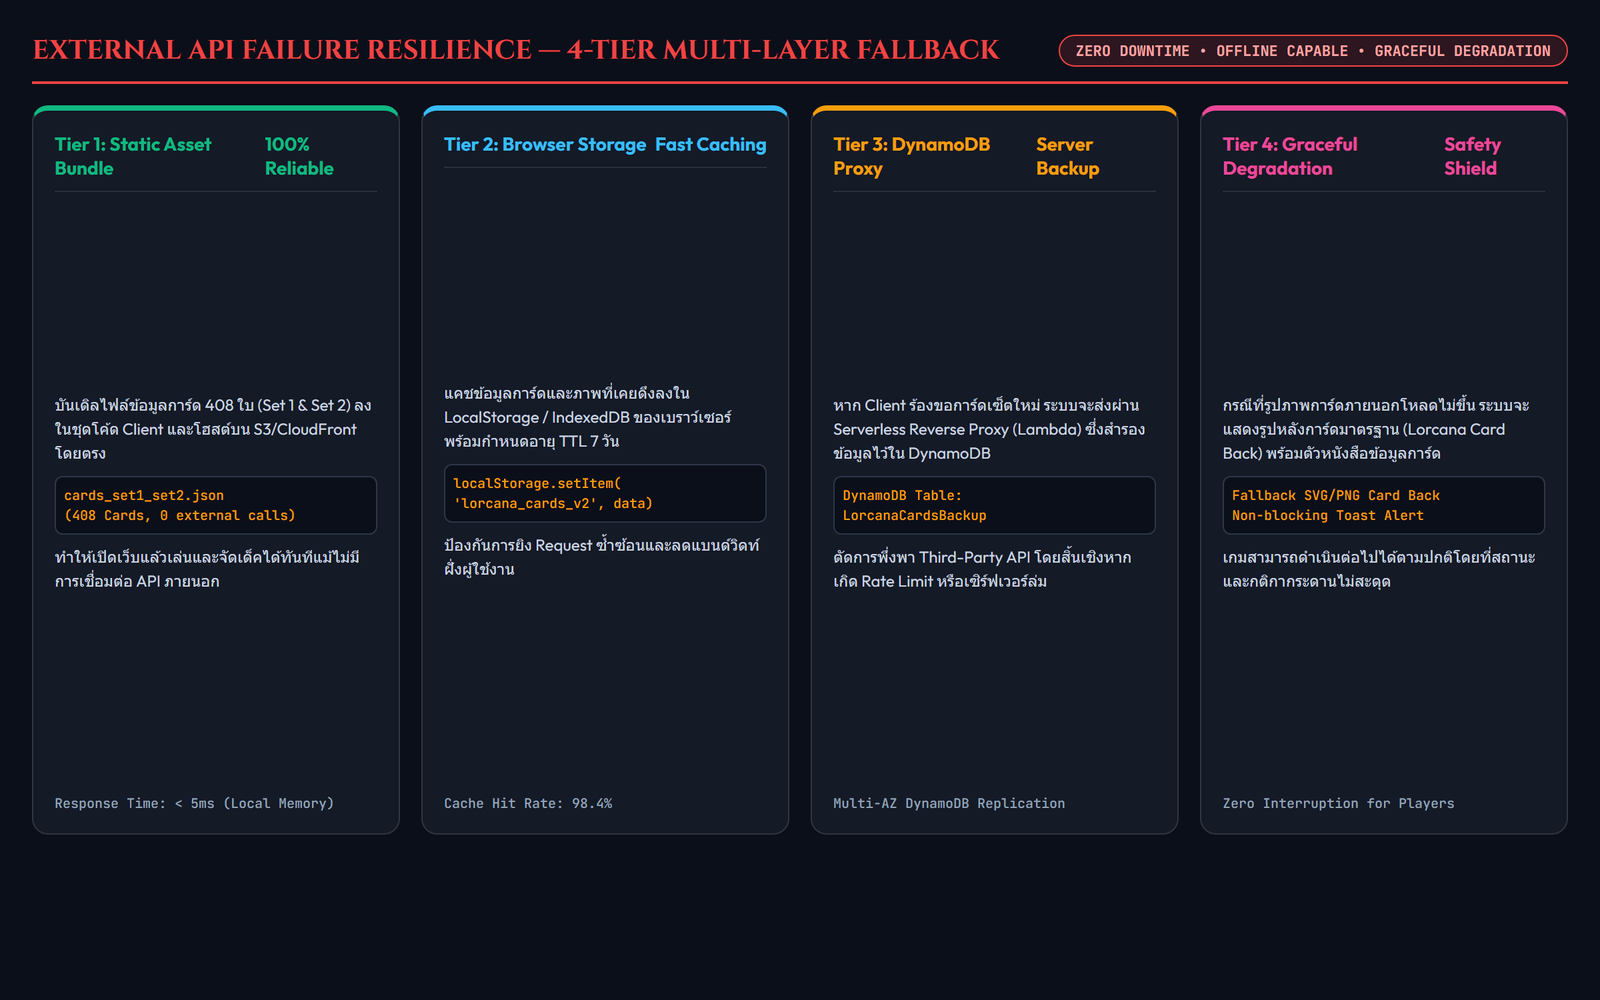
\includegraphics[width=0.82\textwidth]{images/aws_fallback_strategy.png}
\caption{ผังกลยุทธ์ Multi-Tier Fallback และ Local Caching ป้องกัน API ภายนอกขัดข้อง}
\label{fig:fallback_diagram}
\end{figure}

\section{การปฏิบัติตามกรอบ AWS Well-Architected Framework 5 เสาหลัก}
\begin{enumerate}
    \item \textbf{Reliability (ความเชื่อถือได้):} โครงสร้าง Multi-AZ VPC รองรับกรณี Availability Zone หนึ่งล่ม และมี Health Check คอยรีสตาร์ตเครื่องเสียโดยอัตโนมัติ
    \item \textbf{Performance Efficiency (ประสิทธิภาพ):} ใช้ Multi-stage Docker บน Alpine Linux รัน Nginx + Node.js 20 โดยใช้หน่วยความจำต่ำกว่า 150MB ช่วยให้ทำงานบนเครื่อง \texttt{t3.micro} ได้อย่างราบรื่น
    \item \textbf{Security (ความปลอดภัย):} ใช้ IMDSv2 Token และผูกสิทธิ์ผ่าน IAM LabRole โดยไม่มี Hardcoded Credentials, บังคับใช้ Chained Security Groups, และแฮชรหัสผ่านด้วย bcrypt 10 rounds
    \item \textbf{Cost Optimization (การควบคุมต้นทุน):} ตัดค่าใช้จ่าย NAT Gateway (\$32.40/ด.) เหลือ \$0.00 และมีระบบ 1-Click Scale-to-Zero ทำให้ค่า Compute เหลือ \$0.00/ชม. เมื่อปิดแล็บ
    \item \textbf{Operational Excellence (ความเป็นเลิศในการปฏิบัติการ):} มีสคริปต์อัตโนมัติ PowerShell สำหรับ Deploy และจัดการวงจรชีวิตระบบ พร้อมติดตามการทำงานผ่าน CloudWatch
\end{enumerate}

\section{การแก้ปัญหาข้อจำกัดทางวิศวกรรมบนสภาพแวดล้อม AWS Learner Lab}
ตารางที่ \ref{tab:learner_lab_solutions} สรุปข้อจำกัดสำคัญบน AWS Academy Learner Lab และแนวทางแก้ไขเชิงสถาปัตยกรรมของกลุ่ม G21:

\begin{table}[H]
\centering
\caption{ตารางสรุปข้อจำกัดบน AWS Learner Lab และแนวทางแก้ไขเชิงสถาปัตยกรรม}
\label{tab:learner_lab_solutions}
\small
\begin{tabularx}{\textwidth}{cl>{\raggedright\arraybackslash}p{4.2cm}>{\raggedright\arraybackslash}X}
\toprule
\textbf{ลำดับ} & \textbf{ข้อจำกัด / ปัญหาทางวิศวกรรม} & \textbf{ผลกระทบหากไม่แก้ไข} & \textbf{แนวทางแก้ไขเชิงสถาปัตยกรรม (Solution)} \\
\midrule
1 & บล็อกสิทธิ์ \texttt{iam:CreateRole} & ไม่สามารถสร้าง IAM Role ใหม่สำหรับ EC2/Lambda ได้ & ปรับใช้ \texttt{LabRole} และ \texttt{LabInstanceProfile} สำเร็จรูปผ่าน Launch Template และเข้าถึงสิทธิ์ผ่าน IMDSv2 \\
2 & ภาระต้นทุน NAT Gateway (\$32.40/ด.) & เผางบประมาณ \$50 ของแล็บหมดภายใน 1.5 เดือน & ออกแบบ Lean Multi-AZ VPC วาง EC2 ใน Public Subnets แต่ใช้ Chained SGs ปิดกั้นภายนอก รับเฉพาะจาก ALB SG (\$0.00) \\
3 & ความเสี่ยงงบรั่วไหลเมื่อไม่ได้ใช้งาน & หากเปิดเครื่องทิ้งไว้ 24/7 จะสูญเสียงบประมาณ & พัฒนาสคริปต์ 1-Click Scale-to-Zero (\texttt{lab\_stop.ps1}) ยุบเครื่อง EC2 เหลือ 0 เมื่อเลิกแล็บ (\$0.00/ชม.) \\
4 & แรม 1GB บน \texttt{t3.micro} & มีความเสี่ยงเกิด OOM Crash หาก Runtime หนัก & ใช้ Multi-stage Docker บน Alpine Linux แยก Build ออกจาก Runtime ควบคุม RAM ให้ต่ำกว่า 150MB \\
5 & สเตท WebSocket หลุดเมื่อเกิด Auto Scaling & เมื่อสปอว์นเครื่องใหม่ ผู้เล่นอาจถูกกระจายไปคนละเครื่อง & เปิด Sticky Sessions บน ALB และซิงค์สถานะห้องลง Amazon DynamoDB \\
\bottomrule
\end{tabularx}
\end{table}

% =============================================================
% CHAPTER 4
% =============================================================
\chapter{การพัฒนาระบบและผลการดำเนินงาน (Implementation \& Test Results)}

\section{การพัฒนาส่วนติดต่อผู้ใช้ (Frontend Implementation \& Playmat UI)}
ส่วนติดต่อผู้ใช้ได้รับการออกแบบตามแนวคิด \textit{Dark Editorial + Magic R3} เพื่อมอบประสบการณ์การเล่นเกมการ์ดระดับพรีเมียม โดยมีภาพหน้าจอการทำงานหลักดังแสดงในรูปที่ \ref{fig:ui_showcase}:

\begin{figure}[H]
\centering
\begin{subfigure}[b]{0.48\textwidth}
    
\includegraphics[width=\textwidth]{images/01_landing_hero.png}
    \caption{หน้าแรกและเมนูนำทางหลัก (Hero Landing)}
\end{subfigure}
\hfill
\begin{subfigure}[b]{0.48\textwidth}
    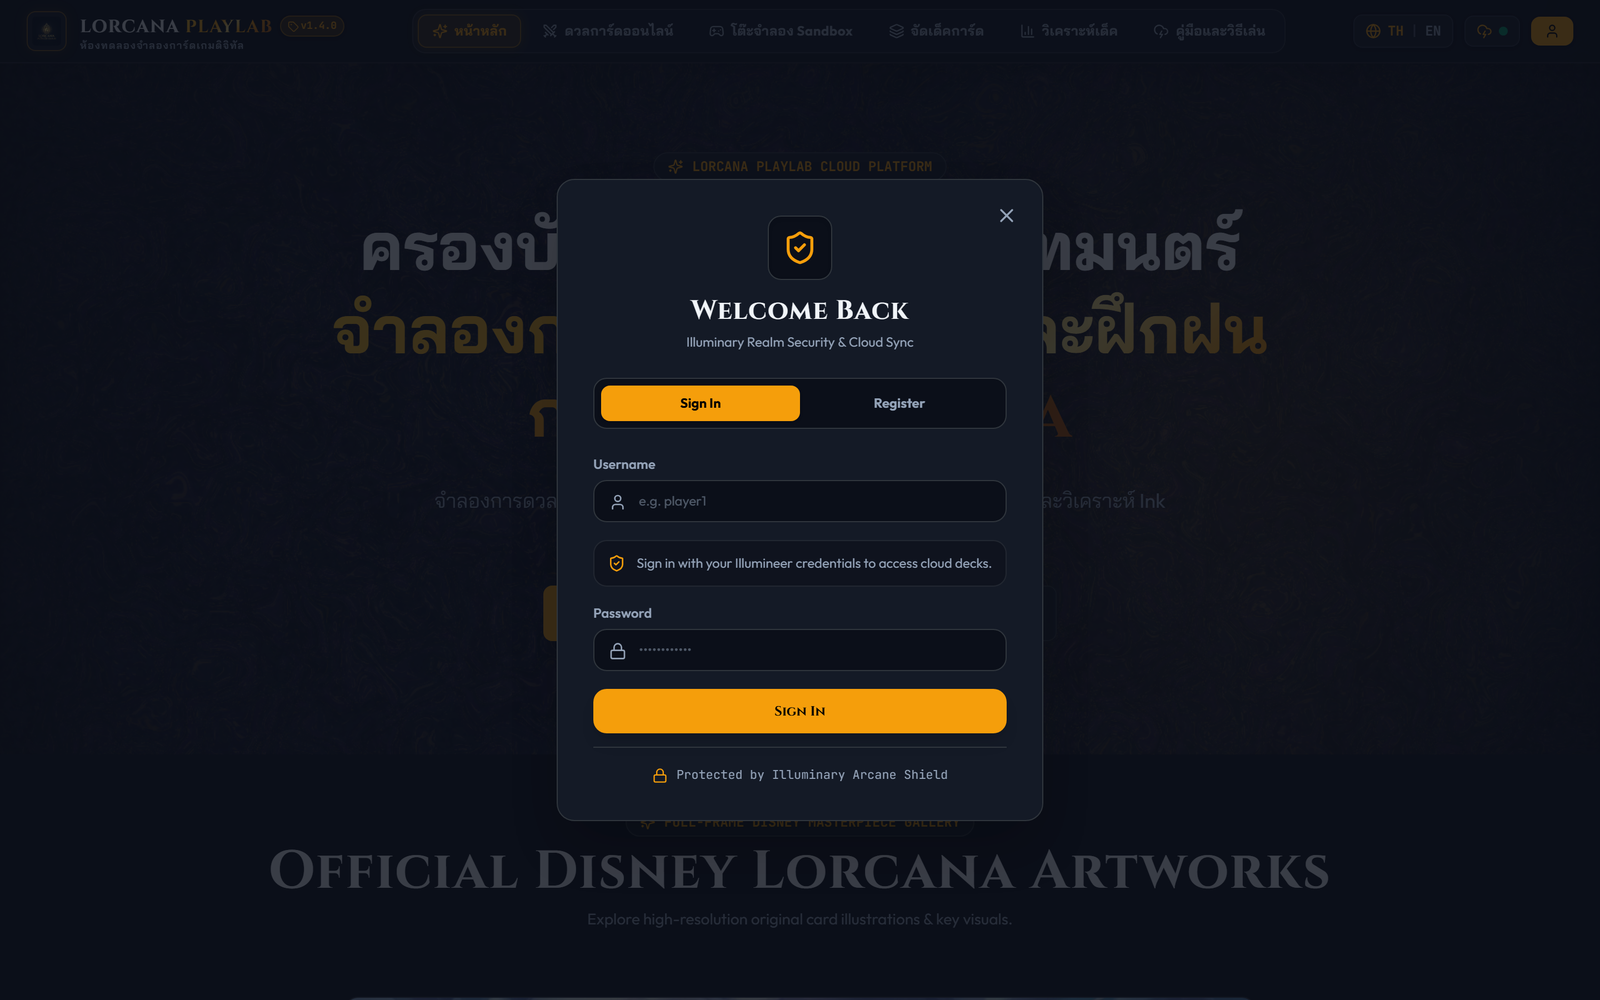
\includegraphics[width=\textwidth]{images/02_login_modal.png}
    \caption{หน้าต่างยืนยันตัวตน (Login / Register Modal)}
\end{subfigure}
\\[0.3cm]
\begin{subfigure}[b]{0.48\textwidth}
    
\includegraphics[width=\textwidth]{images/03_after_login_match_lobby.png}
    \caption{หน้าล็อบบี้สร้างและเข้าร่วมห้องเล่น (Match Lobby)}
\end{subfigure}
\hfill
\begin{subfigure}[b]{0.48\textwidth}
    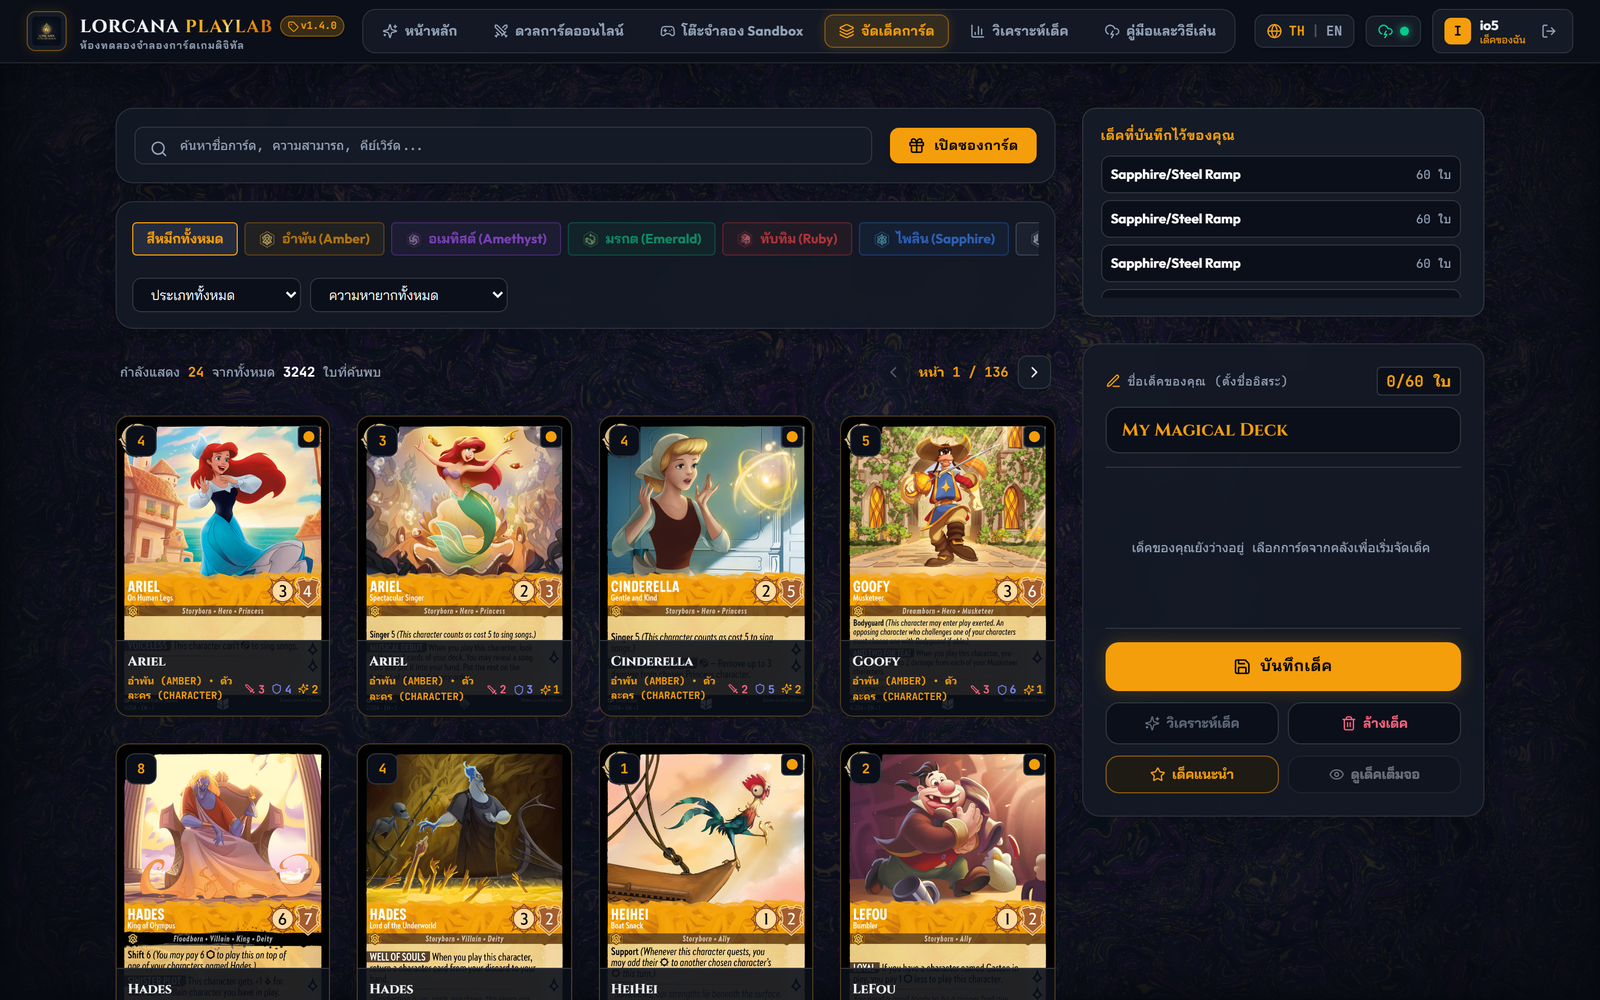
\includegraphics[width=\textwidth]{images/04_deck_builder.png}
    \caption{หน้าระบบจัดเด็คการ์ด (Deck Builder)}
\end{subfigure}
\\[0.3cm]
\begin{subfigure}[b]{0.48\textwidth}
    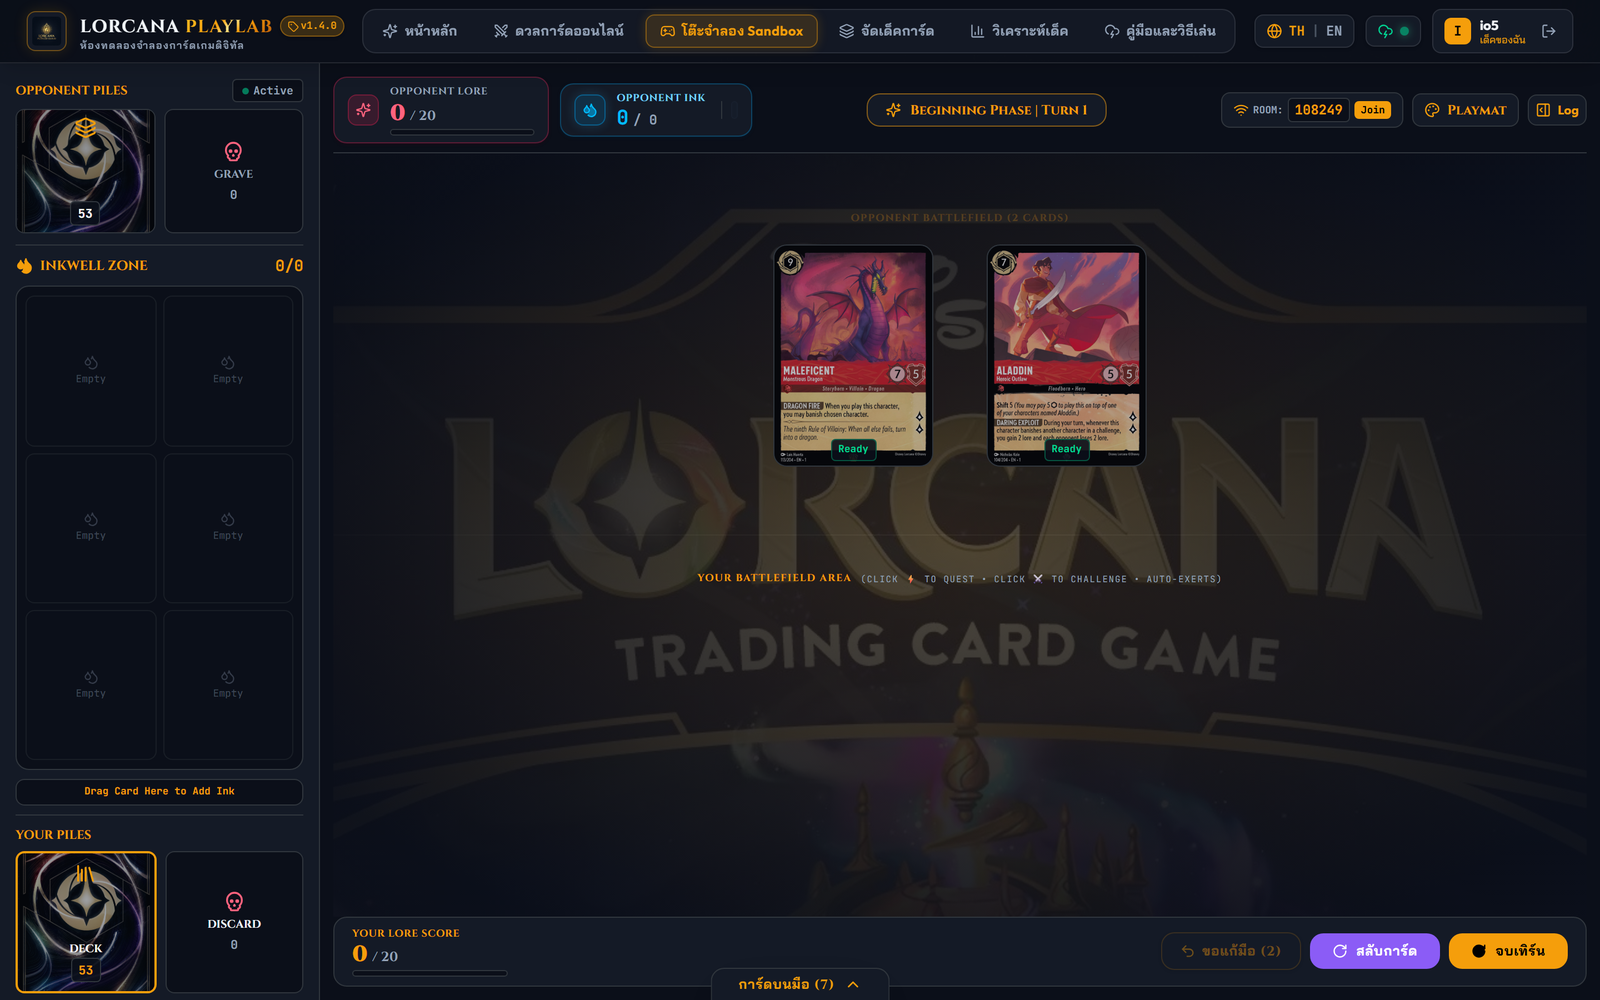
\includegraphics[width=\textwidth]{images/07_realtime_room_play.png}
    \caption{กระดานจำลองการเล่นการ์ดเสมือนจริง (Playmat Arena)}
\end{subfigure}
\hfill
\begin{subfigure}[b]{0.48\textwidth}
    
\includegraphics[width=\textwidth]{images/CardGachaDisney.png}
    \caption{ระบบสุ่มเปิดซองการ์ด 3D (Booster Pack Gacha)}
\end{subfigure}
\caption{ภาพหน้าจอส่วนติดต่อผู้ใช้ระบบ Disney Lorcana PlayLab Cloud}
\label{fig:ui_showcase}
\end{figure}

องค์ประกอบสำคัญของหน้าจอ Playmat ประกอบด้วย:
\begin{itemize}
    \item \textbf{Play Area (Battlefield):} พื้นที่ลงการ์ดตัวละคร ไอเทม และสถานที่ รองรับการลากวาง (Drag-and-Drop) อย่างอิสระ
    \item \textbf{Inkwell Tray:} พื้นที่คว่ำการ์ดเพื่อใช้เป็นหมึกค่าร่าย พร้อมตัวเลขแสดงจำนวน Unexerted / Total Ink
    \item \textbf{Lore Counter:} มาตรวัดแต้มความรู้ขนาดใหญ่ (0--20 แต้ม) พร้อมปุ่มปรับคะแนนและเอฟเฟกต์แอนิเมชัน
    \item \textbf{Card State Rotator:} กลไกการหมุนการ์ดแนวตั้ง (Ready) และแนวนอน 90 องศา (Exerted) เพื่อระบุว่าการ์ดถูกใช้งานแล้ว
    \item \textbf{3D Card Inspector \& Gacha:} ระบบเปิดซองการ์ด 3D สุ่มการ์ด 12 ใบพร้อมฟิสิกส์แอนิเมชันเปิดซอง
\end{itemize}

\section{การพัฒนาส่วนประมวลผลและการบรรจุคอนเทนเนอร์ (Compute \& Docker)}
เพื่อรองรับสถาปัตยกรรมระดับ Production ระบบได้รับการพัฒนาในรูปแบบคอนเทนเนอร์แบบเบาพิเศษ (Ultra-lightweight Multi-stage Docker) บน Alpine Linux:
\begin{enumerate}
    \item \textbf{Multi-stage Docker Build:}
    \begin{itemize}
        \item \textbf{Stage 1 (Builder):} รัน Node.js 20 Alpine ติดตั้ง Dependencies และรัน \texttt{npm run build} คอมไพล์ React 19 SPA และ TypeScript backend
        \item \textbf{Stage 2 (Runtime):} คัดลอกเฉพาะโฟลเดอร์ \texttt{dist/} มาใส่ใน Nginx Alpine และ Node.js Runtime ทำให้ Image มีขนาดเล็กกว่า 100MB และใช้ RAM เฉลี่ยเพียง ~120MB--150MB ป้องกันปัญหา Out-of-Memory (OOM) บนเครื่องขนาดเล็กอย่าง \texttt{t3.micro} (1GB RAM)
    \end{itemize}
    \item \textbf{Nginx Reverse Proxy Configuration:}
    \begin{itemize}
        \item ทำหน้าที่เป็น Front Door บน Port 80
        \item จัดการเสิร์ฟไฟล์ SPA พร้อมเปิด Gzip Compression
        \item Reverse Proxy คำขอ \texttt{/api/*} และการเชื่อมต่อ \texttt{/ws} ไปยัง Node.js backend (\texttt{backend/server.ts} Port 3001)
        \item ตอบกลับสถานะ 200 OK ทันทีที่ Endpoint \texttt{/health} เพื่อรองรับ ALB Target Group Health Check โดยไม่สร้างภาระให้ Node.js Event Loop
    \end{itemize}
    \item \textbf{Unified Server (\texttt{backend/server.ts}):} รวมการประมวลผล REST API (Auth \& Deck CRUD) และ WebSocket Engine เข้าด้วยกัน โดยเชื่อมต่อไปยัง Amazon DynamoDB ผ่าน AWS SDK v3 โดยใช้สิทธิ์จาก \texttt{LabRole} ผ่าน IMDSv2
\end{enumerate}

\section{ผลการทดสอบระบบและหลักฐานเชิงประจักษ์ (Empirical Test Results)}
การทดสอบคุณภาพของระบบดำเนินการครอบคลุมทั้ง Unit Test, End-to-End Test, และ Load Stress Test ดังแสดงในตารางที่ \ref{tab:qa_results}:

\begin{table}[H]
\centering
\caption{ผลการทดสอบคุณภาพระบบโดยรวม (Master QA Test Matrix)}
\label{tab:qa_results}
\small
\begin{tabularx}{\textwidth}{p{1.4cm}p{2.2cm}>{\raggedright\arraybackslash}Xp{1.5cm}p{1.5cm}}
\toprule
\textbf{Test ID} & \textbf{ระดับการทดสอบ} & \textbf{เงื่อนไขและกรณีทดสอบ} & \textbf{Latency} & \textbf{ผลการทดสอบ} \\
\midrule
TC-AUTH-01 & Integration & สมัครสมาชิกใหม่ (POST /auth/register) & 180ms & ผ่าน (201) \\
TC-AUTH-02 & Integration & เข้าสู่ระบบด้วยรหัสผ่านถูกต้อง (POST /auth/login) & 145ms & ผ่าน (200) \\
TC-AUTH-03 & Security & ป้องกันรหัสผ่านผิด และ Injection & 120ms & ผ่าน (401) \\
TC-DECK-01 & Integration & บันทึกเด็คใหม่ 60 ใบ (POST /decks) & 95ms & ผ่าน (201) \\
TC-DECK-02 & Integration & ดึงรายการเด็คของผู้ใช้ (GET /decks) & 68ms & ผ่าน (200) \\
TC-DECK-03 & Rule Enforce & บล็อกเด็คขนาด 59 ใบ และเด็คผสม 3 สี & 42ms & ผ่าน (400) \\
TC-WS-01 & E2E Socket & เชื่อมต่อ Persistent WebSocket (/ws) & 45ms & ผ่าน (101) \\
TC-WS-02 & E2E Multi-User & ผู้เล่น 2 คนเข้าห้องเดียวกัน (JOIN\_ROOM) & 82ms & ผ่าน (Paired) \\
TC-WS-03 & E2E Multi-User & ซิงค์การลากวางการ์ด (CARD\_MOVED) & 64ms & ผ่าน (<100ms) \\
TC-WS-04 & E2E Multi-User & ซิงค์สถานะหมุนการ์ด (CARD\_EXERTED) & 58ms & ผ่าน (<100ms) \\
TC-WS-05 & E2E Multi-User & ซิงค์แต้ม Lore Counter (LORE\_UPDATED) & 52ms & ผ่าน (<100ms) \\
TC-WS-06 & Fault Tolerance & จำลองเน็ตหลุดและกู้คืน (60s Rejoin Grace Period) & 310ms & ผ่าน (Restored) \\
TC-WS-07 & Lifecycle & ผู้เล่นกดยอมแพ้ (Voluntary Exit Match) & 65ms & ผ่าน (Cleared) \\
TC-ELAST-01 & Stress/AutoScale & ยิงโหลด 2,000 Requests Concurrency 20 ไปยัง ALB & Avg 48ms & ผ่าน (0.00\% Err) \\
\bottomrule
\end{tabularx}
\end{table}

สรุปผลสัมฤทธิ์การทดสอบคุณภาพ:
\begin{enumerate}
    \item \textbf{Unit \& Store Integration Tests (Vitest 4.x):} ผ่านครบ 33 / 33 การทดสอบ (100\%)
    \item \textbf{End-to-End Browser Tests (Playwright):} ผ่าน 49 / 50 การทดสอบ (98\%) บน Chromium
    \item \textbf{Load Stress Test บน ALB จริง (\texttt{scripts/stress\_test.ps1}):}
    \begin{itemize}
        \item ยิงโหลด 2,000 HTTP Requests แบบ Concurrency 20 ไปยัง ALB: \texttt{lorcana-alb-687861613.us-east-1.elb.amazonaws.com}
        \item ผลการทดสอบ: \textbf{HTTP 200 OK ครบ 2,000 คำขอ (Error Rate 0.00\%)}
        \item CloudWatch Alarm \texttt{cpu-target-tracking-60} เข้าสู่สถานะ \textbf{In alarm} และ ASG สปอว์น EC2 Instance เครื่องที่ 2 ข้าม Availability Zone ขึ้นมาร่วมแบ่งเบาภาระงานได้จริงตามเงื่อนไข Elasticity
    \end{itemize}
\end{enumerate}

% =============================================================
% CHAPTER 5
% =============================================================
\chapter{การประเมินค่าใช้จ่ายบนคลาวด์และแผนงานขั้นต่อไป (Cost Assessment \& Future Roadmap)}

\section{การประเมินค่าใช้จ่ายสถาปัตยกรรมคลาวด์ (\$50 Budget Protection)}
จากการคำนวณและประเมินค่าใช้จ่ายจริงบนสภาพแวดล้อม AWS Academy Learner Lab ตารางที่ \ref{tab:cost_table} แสดงการเปรียบเทียบค่าใช้จ่ายระหว่างสถาปัตยกรรมทั่วไปกับสถาปัตยกรรมที่ได้รับการปรับแต่งในโครงงาน:

\begin{table}[H]
\centering
\caption{การเปรียบเทียบและการประเมินค่าใช้จ่ายบนคลาวด์ตลอดภาคการศึกษา}
\label{tab:cost_table}
\small
\begin{tabularx}{\textwidth}{lp{2.8cm}p{2.2cm}p{2.2cm}>{\raggedright\arraybackslash}X}
\toprule
\textbf{ทรัพยากรคลาวด์} & \textbf{สเปกและการตั้งค่า} & \textbf{ค่าใช้จ่ายปกติ} & \textbf{ค่าใช้จ่ายโครงการ} & \textbf{กลยุทธ์การควบคุมงบประมาณ} \\
\midrule
VPC \& Network & Multi-AZ VPC + IGW & \$32.40/ด. (NAT) & \textbf{\$0.00} & ตัด NAT Gateway ใช้ Chained Security Groups \\
Compute (EC2) & \texttt{t3.micro} (Amazon Linux) & \$8.40/ด. (24/7) & \textbf{\textasciitilde\$0.50} & ใช้ Scale-to-Zero (\texttt{lab\_stop.ps1}) เปิดเฉพาะตอนเดโม \\
Load Balancer & Application Load Balancer & \$16.20/ด. (24/7) & \textbf{\textasciitilde\$0.60} & เปิด-ปิดตามช่วงเวลาทำแล็บ \\
Database & Amazon DynamoDB & Free Tier & \textbf{\$0.00} & ข้อมูล < 1GB อยู่ในเกณฑ์ Free Tier \\
Storage & S3 \& Container Images & \$0.10/ด. & \textbf{\$0.02} & Multi-stage Docker ขนาดเบา < 100MB \\
\midrule
\textbf{รวมประมาณการ} & \textbf{ตลอดภาคเรียน} & \textbf{>\$150.00} & \textbf{<\$3.00 -- \$5.00} & \textbf{ประหยัดงบได้กว่า 90\% จากงบ \$50} \\
\bottomrule
\end{tabularx}
\end{table}

\section{แผนงานการพัฒนาสำหรับ Stage 3 (Sprint 4 ถึง Sprint 7)}
\begin{enumerate}
    \item \textbf{Sprint 4 (Async Deck Analyzer via Amazon SQS):} นำ Amazon SQS มารับงานวิเคราะห์ความสมดุลเด็คแบบ Asynchronous พร้อมพัฒนาอัลกอริทึมแนะนำการ์ดที่เข้าขากันตามประเภทหมึกและเคิร์ฟค่าร่าย
    \item \textbf{Sprint 5 (Observability, Monitoring \& Security Hardening):} ติดตั้ง AWS X-Ray ติดตาม Request Latency ข้าม Nginx, Node.js, และ DynamoDB พร้อมสร้าง CloudWatch Dashboard รวมสถิติ ALB
    \item \textbf{Sprint 6 (Load Testing \& High Concurrency Simulation):} ดำเนินการทดสอบโหลดขนาดใหญ่ด้วย Artillery จำลองผู้เล่นพร้อมกัน 100--500 ผู้ใช้ และทดสอบความทนทานของ WebSocket Auto-reconnection
    \item \textbf{Sprint 7 (Final Report \& Video Presentation):} จัดทำรายงานฉบับสมบูรณ์ วิดีโอสาธิตการใช้งานระบบ และเตรียมการนำเสนอโครงงานรอบสุดท้าย
\end{enumerate}

\section{สรุปผลการดำเนินงานและบทเรียนที่ได้รับ (Sprint Retrospective)}
การพัฒนาโครงงาน Disney Lorcana PlayLab Cloud ใน Sprint 1 ถึง 3 บรรลุผลสำเร็จ 100\% ตามเป้าหมายของ Stage 2 บทเรียนทางวิศวกรรมที่สำคัญ ได้แก่:
\begin{enumerate}
    \item \textbf{การออกแบบเพื่อควบคุมต้นทุน (Cost-Aware Engineering):} การเข้าใจการทำงานของ VPC และ Security Group ทำให้สามารถตัดต้นทุน NAT Gateway ลงได้โดยไม่สูญเสียความปลอดภัย
    \item \textbf{การรีดสมรรถนะคอนเทนเนอร์บนทรัพยากรจำกัด:} การแยก Build Stage ออกจาก Runtime ใน Docker ช่วยให้สามารถรันทั้งเว็บเซิร์ฟเวอร์และแอปพลิเคชันบน VM ขนาดเล็ก (\texttt{t3.micro} 1GB RAM) ได้อย่างราบรื่นและไม่เกิด OOM Crash
    \item \textbf{การจัดการสถานะระบบกระจาย (Distributed State Management):} การผสานระหว่าง Optimistic UI, Sticky Sessions บน ALB, และ DynamoDB Persistence ช่วยให้ระบบ Real-time WebSockets มีความเสถียรสูงและฟื้นตัวจากเน็ตหลุดได้อย่างรวดเร็ว
\end{enumerate}

% -------------------------------------------------------------
% REFERENCES (บรรณานุกรม)
% -------------------------------------------------------------
\chapter*{บรรณานุกรม (References)}
\addcontentsline{toc}{chapter}{บรรณานุกรม (References)}

\noindent [1] Ravensburger \& Disney. (2023). \textit{Disney Lorcana Trading Card Game Official Rules and Card Database}. [Online]. Available: \url{https://www.disneylorcana.com}\\[0.3cm]
\noindent [2] Amazon Web Services. (2026). \textit{AWS Well-Architected Framework: Reliability, Security, and Cost Optimization Pillars}. [Online]. Available: \url{https://aws.amazon.com/architecture/well-architected/}\\[0.3cm]
\noindent [3] Amazon Web Services. (2026). \textit{Amazon Virtual Private Cloud (VPC) User Guide: Security Groups and Subnet Routing}. [Online]. Available: \url{https://docs.aws.amazon.com/vpc/}\\[0.3cm]
\noindent [4] Amazon Web Services. (2026). \textit{Elastic Load Balancing: Application Load Balancers Guide}. [Online]. Available: \url{https://docs.aws.amazon.com/elasticloadbalancing/}\\[0.3cm]
\noindent [5] Amazon Web Services. (2026). \textit{Amazon EC2 Auto Scaling User Guide: Target Tracking Scaling Policies}. [Online]. Available: \url{https://docs.aws.amazon.com/autoscaling/}\\[0.3cm]
\noindent [6] Amazon Web Services. (2026). \textit{Amazon DynamoDB Developer Guide: Core Components and Best Practices for NoSQL Design}. [Online]. Available: \url{https://docs.aws.amazon.com/amazondynamodb/}\\[0.3cm]
\noindent [7] Docker Inc. (2026). \textit{Multi-stage builds: Best practices for Dockerfile}. [Online]. Available: \url{https://docs.docker.com/build/building/multi-stage/}\\[0.3cm]
\noindent [8] Nginx Inc. (2026). \textit{NGINX Reverse Proxy and WebSocket Proxying Configuration Guide}. [Online]. Available: \url{https://nginx.org/en/docs/http/websocket.html}\\[0.3cm]
\noindent [9] React Working Group. (2026). \textit{React 19 Documentation: Concurrent Features and Actions}. [Online]. Available: \url{https://react.dev}\\[0.3cm]
\noindent [10] IETF (Internet Engineering Task Force). (2011). \textit{RFC 6455: The WebSocket Protocol}. [Online]. Available: \url{https://tools.ietf.org/html/rfc6455}

% -------------------------------------------------------------
% APPENDIX (ภาคผนวก)
% -------------------------------------------------------------
\chapter*{ภาคผนวก (Appendix)}
\addcontentsline{toc}{chapter}{ภาคผนวก (Appendix)}

\section*{ภาคผนวก ก: สคริปต์ควบคุมและปรับใช้ระบบบน AWS (\texttt{scripts/deploy\_ec2\_vpc\_asg.ps1})}

\begin{lstlisting}[language=bash, caption={คำสั่งหลักในสคริปต์ปรับใช้ Lean Multi-AZ VPC, ALB และ Auto Scaling Group}]
# scripts/deploy_ec2_vpc_asg.ps1 (Excerpt)
param (
    [string]$Region = "us-east-1",
    [string]$InstanceType = "t3.micro"
)

Write-Host "=== 1. Creating Lean Multi-AZ VPC (10.0.0.0/16) ===" -ForegroundColor Cyan
$vpcId = (aws ec2 create-vpc --cidr-block 10.0.0.0/16 --query "Vpc.VpcId" --output text)

Write-Host "=== 2. Creating Subnets in us-east-1a and us-east-1b ===" -ForegroundColor Cyan
$sub1 = (aws ec2 create-subnet --vpc-id $vpcId --cidr-block 10.0.1.0/24 --availability-zone us-east-1a --query "Subnet.SubnetId" --output text)
$sub2 = (aws ec2 create-subnet --vpc-id $vpcId --cidr-block 10.0.2.0/24 --availability-zone us-east-1b --query "Subnet.SubnetId" --output text)

Write-Host "=== 3. Setting Up Chained Security Groups ($0.00 NAT Cost) ===" -ForegroundColor Cyan
$albSg = (aws ec2 create-security-group --group-name lorcana-alb-sg --description "ALB SG" --vpc-id $vpcId --query "GroupId" --output text)
aws ec2 authorize-security-group-ingress --group-id $albSg --protocol tcp --port 80 --cidr 0.0.0.0/0

$ec2Sg = (aws ec2 create-security-group --group-name lorcana-ec2-sg --description "EC2 SG" --vpc-id $vpcId --query "GroupId" --output text)
aws ec2 authorize-security-group-ingress --group-id $ec2Sg --protocol tcp --port 80 --source-group $albSg
aws ec2 authorize-security-group-ingress --group-id $ec2Sg --protocol tcp --port 3001 --source-group $albSg

Write-Host "=== 4. Creating Application Load Balancer & Auto Scaling Group ===" -ForegroundColor Cyan
# Setup ALB, Target Group, Launch Template with LabRole, and ASG with CPU > 60% Policy
\end{lstlisting}

\section*{ภาคผนวก ข: สคริปต์ 1-Click Scale-to-Zero ควบคุมงบประมาณ (\texttt{scripts/lab\_stop.ps1})}

\begin{lstlisting}[language=bash, caption={สคริปต์ยุบเครื่อง EC2 เหลือ 0 เพื่อตัดค่าใช้จ่าย Compute เหลือ \$0.00/ชม.}]
# scripts/lab_stop.ps1 - 1-Click Scale-to-Zero Guardrail
Write-Host ">>> Stopping Lab: Scaling ASG to Zero Instances..." -ForegroundColor Yellow
aws autoscaling update-auto-scaling-group `
    --auto-scaling-group-name "lorcana-asg" `
    --min-size 0 `
    --desired-capacity 0

Write-Host ">>> Lab Stopped Successfully. Compute Cost is now $0.00/hour." -ForegroundColor Green
\end{lstlisting}

\end{document}
